\section*{Podstawy rachunku wektorowego}

    Podstawowe działania na wektorach, które będą potrzebne w toku zajęć z Mechaniki Technicznej, to:
    \begin{itemize}
        \item iloczyn skalarny,
        \item iloczyn wektorowy,
        \item moment siły względem punktu.
    \end{itemize}

    \subsection*{Przykład}
    Oblicz moment siły \textbf{P} względem punktu C.
    
    \begin{figure}[H]\centering
        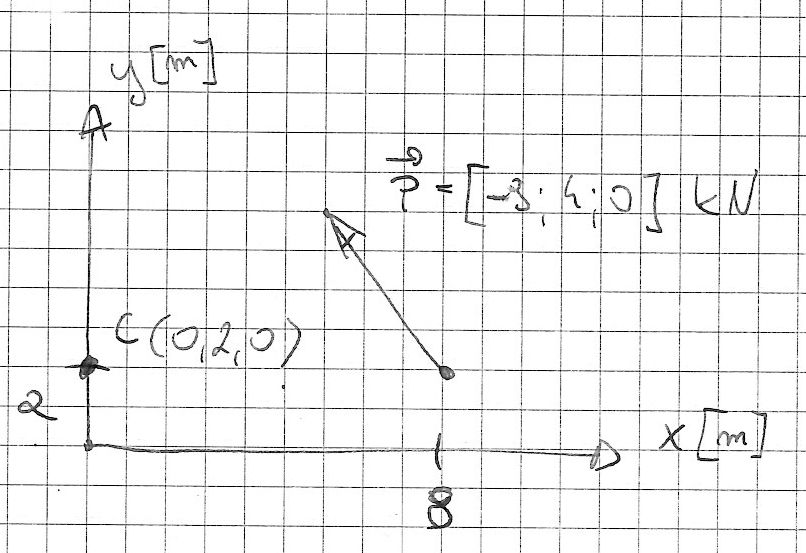
\includegraphics{01-moment_sily.jpg}
        \caption{Położenie głównych centralnych osi bezwładności przekroju}
    \end{figure}
    
    \begin{equation}
        \textbf{M}_c = \sum_{j=1}^m \textbf{M}_j + \sum_{i=1}^n \textbf{r}_{ci} \times \textbf{P}_i
    \end{equation}